\subsection{Архитектура приложения и структура файлов}
В процессе разработки приложения была использована следующая структура папок, определяющая архитектуру и обеспечивающая удобство и наглядность организации кода:
\begin{itemize}
    \item Properties: В этой папке хранятся классы, предоставляющие механихм хранения настроек пользователя, которые необходимо хранить между сеансами работы с приложением. А также файл Resources.resx, который служит для хранения всех строковых ресурсов, используемых в приложении.

    \item Behaviors: Данная папка содержит классы, реализующие поведения элементов пользовательского интерфейса, такие как валидация вводимых данных, обработка событий и другие специфические для конкретного элемента поведения.

    \item Controls: В этой папке хранятся пользовательские элементы управления, разработанные специально для данного приложения. Они расширяют стандартные элементы управления, предоставляемые фреймворком MAUI, и добавляют дополнительную функциональность или внешний вид, необходимые для реализации требований приложения.

    \item Converters: Папка Converters содержит классы конвертеров, используемые для преобразования значений между различными типами данных или форматами. Они используются для обеспечения связывания данных между моделями и представлениями.

    \item Helpers: В папке Helpers находятся вспомогательные классы, предоставляющие общие функции, которые могут быть использованы в разных частях приложения, такие как утилиты для работы с датами, строками, файлами и другими.

    \item Models: Папка Models содержит классы, описывающие основные сущности и структуры данных приложения, такие как врачи, медицинские карты и другие объекты, а также связи между ними.

    \item Platforms: В этой папке располагается код, специфичный для определенных платформ (например, Android, iOS, Windows). Он позволяет адаптировать приложение под различные платформы, учитывая их особенности.

    \item Resources: Папка Resources содержит файлы ресурсов, такие как изображения, строки, стили и цветовые схемы, используемые в приложении.

    \item Services: В папке Services хранятся классы, реализующие различные сервисы, необходимые для работы приложения, такие как сервисы для работы с API сервера, сервисы доступа к данным и другие.

    \item Triggers: Папка Triggers содержит классы триггеров, которые используются для изменения свойств или применения стилей к элементам пользовательского интерфейса в ответ на определенные условия или события.

    \item ViewModels: В папке ViewModels находятся классы моделей представления (ViewModels), реализующие логику приложения, связанную с представлениями. В этих классах выполняется обработка пользовательского ввода, обеспечивается связывание данных с представлениями и координация действий между различными слоями приложения.

    \item Views: Папка Views содержит файлы разметки и кода, описывающие представления пользовательского интерфейса приложения. В этих файлах определяются элементы управления, их расположение и стили, а также связывание с моделями представления для обеспечения интерактивности и обновления данных на экране.
\end{itemize}

На рисунке~\ref{fig:fig02} представлена данная архитектура.
\begin{figure}
  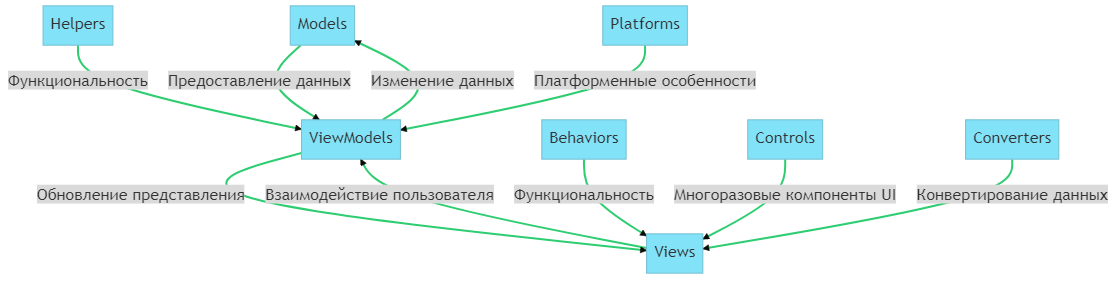
\includegraphics[scale=0.5]{inc/architecture.png}
  \caption{Архитектура приложения}
  \label{fig:fig02}
\end{figure}

Важным аспектом архитектуры приложения является корректная обработка ошибок и исключений. В приложении используются следующие подходы:
\begin{enumerate}
    \item Централизованная обработка ошибок: Обработка ошибок на уровне сервисов и моделей представления обеспечивает единый механизм обработки исключений, а также предотвращает распространение ошибок на уровень представлений.

    \item Использование пользовательских исключений: Для обработки специфических ошибок, связанных с логикой приложения, созданы пользовательские исключения, которые облегчают отслеживание и обработку ошибок в различных частях программы.

    \item Надежная работа с ресурсами: При работе с ресурсами, такими как файлы, сетевые соединения или базы данных, используются конструкции, обеспечивающие безопасное освобождение ресурсов в случае ошибки. Например, оператор using в C\# гарантирует корректное закрытие потоков или соединений с базой данных.
\end{enumerate}

Для обеспечения высокой производительности и отзывчивости приложения, были разнообразные подходы. К примеру, асинхронное программирование - операции, которые могут вызывать блокировку выполнения, такие как доступ к базе данных или сетевым ресурсам, выполняются асинхронно с использованием ключевых слов async и await. Это позволило приложению оставаться отзывчивым во время выполнения длительных операций. Также применяются виртуализация и ленивая загрузка данных, что позволяет загружать и отображать только те элементы, которые находятся в видимой области экрана и индексирование полей таблиц базы данных для ускорения получения результатов на запрос. 

Соблюдение всех вышеуказанных принципов и практик позволяет создавать надежное, производительное и легко расширяемое приложение для заполнения медицинской карты отделения неотложной медицинской помощи